\subsection{Approximating NMF with STDPH}
% The paragraphs here describing why NSC might be all over the place seems out of place in a section that should focus on STDPH's ability to approximate NMF. Thinking of cutting this and moving it into the discussion.
% --------------------------------------
% The brain may have adopted \ac{NSC} as a ubiquitous coding strategy throughout the brain because \ac{NSC} imbues it with two desirable, and perhaps critical, properties. Firstly, sparsity has been shown to be important for energy conservation, and since the brain already consumes more of the body's energy resources than any other organ  (up to 20\%) CITATION NEEDED?, it is likely important for neurons to have an energy-efficient way of handling the sheer number of inputs it receives on a day-to-day basis. It has also been noted that despite its high energy expenditure, the brain is remarkably power efficient (this paper might be a good citation: http://ieeexplore.ieee.org/abstract/document/6797884/).
% Secondly, nonnegativity is an already intuitive constraint for neurons whose firing rates cannot be negative, and furthermore, nonnegativity may give rise to a parts-based, rather than a holistic, method of representation (note: this paints a more simplistic picture than what may actually be the case, since a neuron's inhibitory inputs can effectively cancel out the influence of other inputs; see Bar-Gad...) . %The following assumes you already agree that SOME FORM of dimensionality reduction occurs, otherwise it's easy to say 'well it's not any of these' :
% Parts-based representations are weighted more evenly than representations that might result from dimensionality reduction techniques like PCA, in which most of the variance is captured by the first couple of components and every subsequent component explains less of the variance. This means that some neurons encapsulate more information about stimuli than others, and if they are damaged, other neurons would be less able to compensate for the loss. In a parts-based representation, each part can contribute equally, so the loss of one neuron is not catastrophic for the system.
% --------------------------------------

% \mikeNote{words whole para}
% What might be the reason that we find \ac{NSC} all over the brain?
% % For one, confirmation bias (haha)
% For one, \ac{NSC} might possess properties that are desirable by a biological
% system, such as sparsity (for energy saving)
% and the parts-based representation
% (since in a holistic representation,
% if you knock out the principal component, you're screwed).
% Wouldn't you emphasize the redundancy thing here more than that? It seems to me that if you knocked out a parts-based representation it'd still be just as bad as if it was holistic , but one thing that really stood out to me in the retina and early visual papers is that NMF creates really stable representations because it pulls out broad consistences in activation that creates a stereotyped pattern of activation, whereas other statistical constraints like PCA or ICA actually pull out inconsistencies in neuronal activation and since it emphasizes the differences, representations are less stable/robust. It seems to me that if this is the case and you knocked neurons out, you could lose important amplified differences that each 'basis' brought to the representation, whereas with NMF since it encapsulates stereotypy you lose less information overall if you lose a neuron.
%
% If you can boil this down to a short sentence or two, I'd probably buy it!
% I just don't understand what this actually means:
% "pulls out broad consistences in activation that creates a stereotyped pattern 
% of activation". Consistent/stereotyped with respect to what?
% The point I was trying to make was much simpler. In NMF, every basis function has roughly
% the same weight/importance (not for a particular stimulus, but over the whole lifetime).
% In PCA, the first principal component explains say 50% of the variance, and the second
% component actually only explains stuff the first can't.
% Thus in PCA there's a dependence between components. In NMF (or actually in ICA)
% not so much. - Mike

\mikeNote{The narrative needs some work here. In para 1 we propose STDPH == NSC. In para 2 we have proof for it through Carlson (so no need to propose anything). In para 3 we investigate whether it's true. I suggest reordering so that we say: 1) we have reason to believe NSC == STDPH. 2) STDPH is this and that. 3) we investigated this further with our experiment }
That \ac{NSC} can explain and reproduce response properties observed in biological neurons may be an important clue as to how brains have evolved to parse and store information. One candidate \ac{NSC} process in the brain is synaptic plasticity, 
which may act on synapses for the purpose of reducing dimensionality on an input space in order to represent it efficiently and sparsely, the same as \ac{NSC}. Specifically, we
propose that \ac{NSC} might be functionally equivalent to \ac{STDPH}. STDP is a spike timing based correlative learning rule in which the
timing of the pre- and post-synaptic spikes determining the sign
\mikeNote{explained LTP, LTD}
(i.e., long-term depression or long-term potentiation)
and amplitude of synaptic weight changes \citep{BiPoo1998,SongAbbott2000}.
It acts on specific synapses over a short time scale 
(i.e., milliseconds to seconds). Homeostasis, which keeps neuronal activity in a good working range, acts over a longer timescale (i.e., minutes to days) and is applied to multiple synapses on a neuron or over multiple neurons \citep{turrigiano1998}.  Homeostasis also facilitates synaptic competition by normalizing the inputs to a neuron. This evens the playing field for synapses that weaken due to imbalances in activity, but might otherwise strengthen if left to their own devices \citep{chistiakova2015}.

Experimental and theoretical evidence suggest that biological processes, such as synaptic plasticity and homeostatic mechanisms, may be reducing the dimensionality of inputs in a similar way to NMF. For example, Carlson and colleagues \citep{Carlson2013} delivered a mathematical proof
that \ac{STDPH} can approximate the \ac{NMF} algorithm (Box 2).
Similar to Oja's rule \citep{Oja1982}, which was developed to stabilize 
rate-based Hebbian learning
(effectively resulting in \ac{PCA}),
synaptic scaling acts as a homeostatic mechanism to stabilize \ac{STDP}
(effectively resulting in \ac{NMF}).
This finding suggests that neurons are able to find accurate factorial
representations of their input stimulus spaces through means of Hebbian-like
synaptic learning. In addition, sparsity of the encoding might be enforced by spike thresholding \citep{Rozell2008}
and lateral inhibitory connections \citep{Coultrip1992}.

To investigate this equivalence
\mikeNote{added the bit on the setting}
in a more realistic setting,
we conducted simulations in which a model based on \ac{STDPH} and a model based on \ac{NSC} were applied to a dataset of recorded neuronal activity observed in the \ac{RSC} of rats in a spatial navigation task. In this task, rats ran back and forth on a W-shaped track that could occupy different spatial locations within the room. During the experiment,
activity from 228 \ac{RSC} neurons 
was recorded along with four behavioral metrics: linear velocity, angular velocity, head direction, and allocentric position. Using Gaussian and cosine tuning curves, we created idealized input neurons that encoded these four variables. For the \ac{STDPH} experiment, the idealized input neurons generated spike trains as input to a population of SNNs that were trained using an evolutionary strategy (Box 3) to match the recorded electrophysiological data \citep{Rounds2016}. 

\mikeNote{IMO these following paras are much too detailed. I think the EA details distract from the main argument, and don't add much value for the general understanding. The reader doesn't need to understand binary tournament selection, crossover, and mutation to appreciate the fact that you were able to fit SNN activity to neurophysiological recordings. Also now the glossary is 44\% EAs.}
In these experiments, the
\mikeNote{What population?}
population size was $N = 15$. We randomly selected trials from a pool containing half the trials in the dataset for training (the other half were reserved for the testing phase). The testing phase was the same as the training phase except STDPH was disabled. Following testing, we measured correlations between synthetic and electrophysiological activity patterns and chose synthetic neuronal matches for each experimentally observed firing pattern based on the best correlations between them. Following fitness evaluation, we used
\mikeNote{IMO could be shortened. ``We used an evolutionary strategy (binary tournament selection, mutation without crossover) implemented in CARLsim [REF] and ECJ [REF] to match this to that.'' or similar. }
\textbf{binary tournament selection} to choose three new parents (each parent produced five children) for the next generation of individuals. Each new parent underwent mutation without crossover to produce a new child.
To compare experimental neuronal responses with synthetic ones, we analyzed functional neuron types using methods described in Alexander and Nitz \citep{AlexanderNitz2015}. Activations averaged over trials for every neuron in the population were cross-correlated to reconstruct agent’s position within a route. To reconstruct position with respect to one route (such as in 
\mikeNote{Please first explain what $\alpha$ and $\beta$ are. L and R are a bit easier to guess}
$\alpha$LRL), trials were divided into two sets, even and odd, to measure consistency of response. To reconstruct position between track positions (such as in $\alpha$$\beta$LRL), activations over trials associated with the $\alpha$ track position were averaged and cross-correlated with averaged activations over trials associated with $\beta$. High correlations between same positions (e.g., bin 1 (row) and bin 1 (column)) indicate a good reconstruction of position from ensemble activity
\mikeNote{add ``see Fig. X, Y'' etc.?}
patterns. Within-position reconstructions (even vs. odd trials) yielded accurate positional reconstructions (low error), but between-position (i.e., $\alpha$ vs. $\beta$ trials) were associated with high error and did not yield accurate reconstructions of position, which suggests that the population differentiates routes situated in different parts of space.
The evolutionary algorithm was used to optimize STDPH parameters in the model, corresponding to the temporal window over which spike times were integrated, the amount each synaptic weight increased or decreased, and the target baseline firing rates of excitatory and inhibitory neurons. During each generation of the evolutionary run, models were trained on trials randomly selected from half of the available dataset, then tested on trials randomly selected from the latter half reserved for testing. At the end of each generation, synthetic neural activity was correlated with electrophysiologically recorded neural activity, which served as the fitness metric for the algorithm. After the model finished an evolutionary run, SNN activity closely matched the electrophysiological activity. For the \ac{NSC} experiment, we constructed an input matrix containing half the trials associated with the task to be used as a training set, in which each row was one of the four behavioral metrics, and each column was associated with an element in one of the recorded trials. We applied \ac{NMF} to the input matrix and then used the remaining half of the trials to test the model and gather responses from the model neurons.

We found that the activity patterns of both \ac{NSC} and \ac{STDPH} model neurons could replicate the neuronal response properties and ensemble activity seen in the electrophysiologically recorded neurons in the dataset (Fig.~\ref{fig:NMF|RSC}A, B, C, left); that is, the model neuron activity could be classified into three broad categories,
with remarkably similar population statistics to rat \ac{RSC} 
\citep{AlexanderNitz2015}:
1) Turn-sensitive, no modulation neurons responded whenever the animal made a left or right turn
   on the track (light gray);
2) Turn-sensitive, route modulation neurons responded whenever the animal made a turn on a specific position along
   the route, independent of allocentric location (dark gray); and
3) Turn-insensitive neurons that could not be classified according to the above,
   but nonetheless exhibited complex and robust firing patterns (white). In addition, both \ac{NSC} and \ac{STDPH} model \ac{RSC} produced simulated neurons whose ensemble activity vectors could be used to predict the agent's location on a route with respect to the allocentric frame of reference. Ensemble activity patterns could also disambiguate the agent's location within routes that occupied different locations in the room, consistent with findings of population behavior in the biological RSC \citep{AlexanderNitz2015}. When same-track position trials were correlated, ensemble prediction error was very low, but when conflicting-track position trials were correlated, prediction error was significantly higher in all cases (Fig.~\ref{fig:NMF|RSC}A, B, C, right); for further details on this analysis, see \citep{AlexanderNitz2015,Rounds2016}.
   
% \mikeNote{Figure 3 caption: I still have a hard time understanding this figure. You never say what LRL and RLR means (although I can guess), or what the difference/significance of ``even'' vs ``odd'' trials is.  Alternatively, could we find a more intuitive (i.e., human-readable) labeling of the different track configurations (across/within tracks, same track across trials, or similar)? Otherwise seems a bit overly complicated for this high-level article.}
% \emilyNote{See new method box 3.}

% \jeffNote{Re-write Fig.3 caption. First explain left versus right columns. Define terms (alpha, beta, LRL, etc. Then all that is needed to say is A. Experimental data from Alexander \& Nitz. B. Simulated using NMF. C. Simulated by evolving STDPH parameters to fit experimental data from Rounds et al.).}


% \jeffNote{I think the Figure 3 caption could be drastically shortened. The relevant details are in the text. Explain a is experimental,b is NMF, and c is STDPH with REFS. Explain the labels. Then say see text for details.}
\begin{figure}[ht]
	\centering
	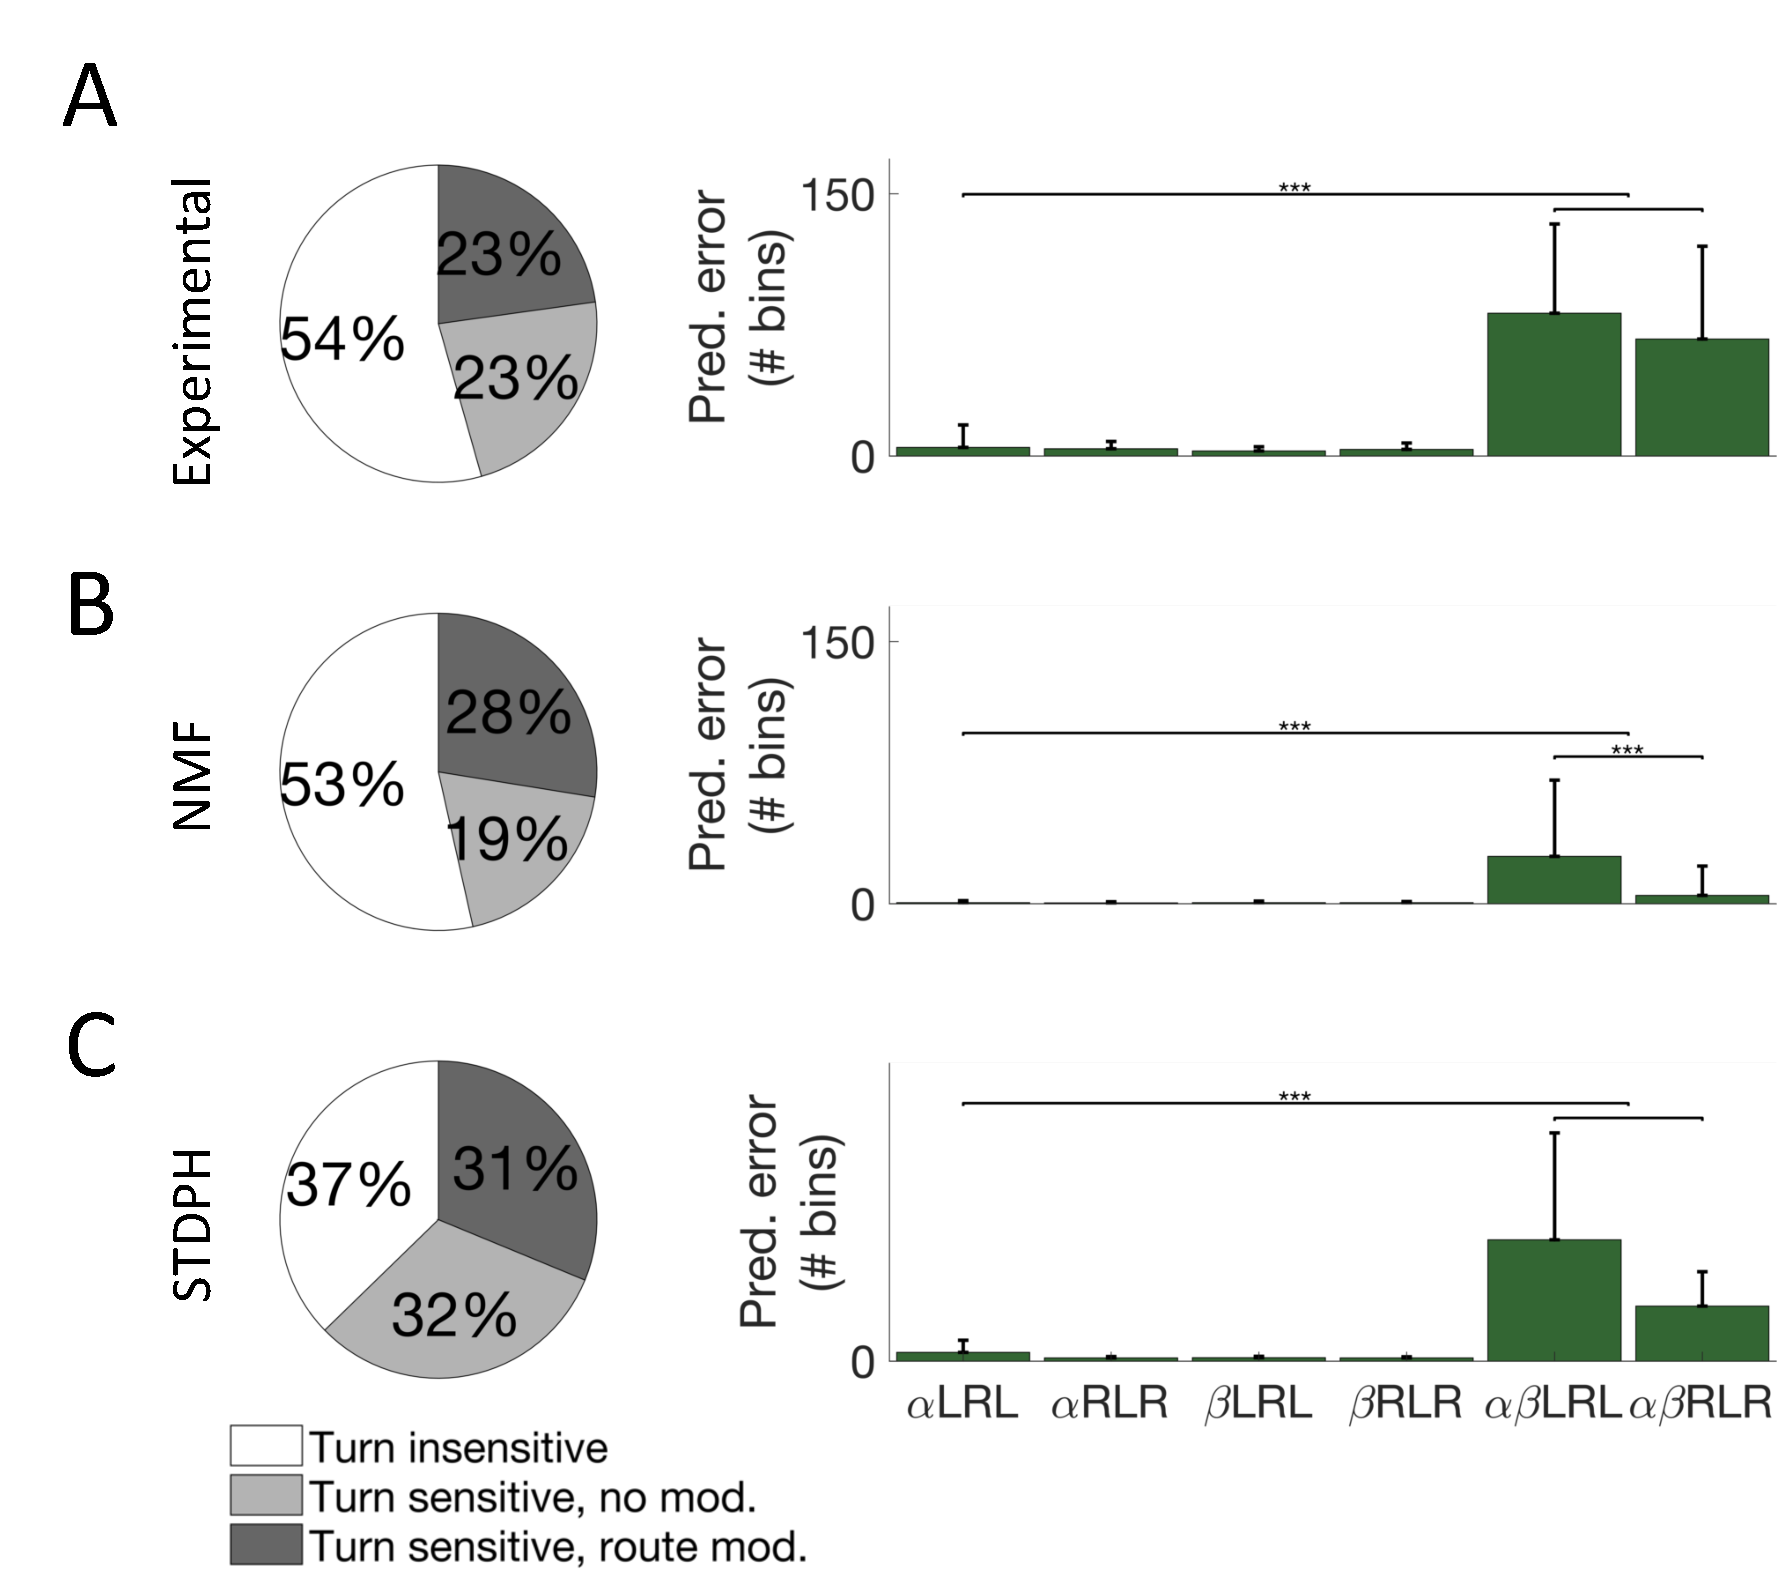
\includegraphics[width=\textwidth]{fig3}
    \caption{Functional neuron type distributions found in the dataset and produced by each model (left columns) and average error corresponding to positional ensemble reconstruction matrices (right columns). Separate allocentric positions of the track are represented by the symbols $\alpha$ and $\beta$. Reconstructions between the track positions are represented by $\alpha$$\beta$. There were two possible routes associated with each track: an outbound run consisting of a left-right-left (LRL) turn sequence and an inbound run consisting of a right-left-right (RLR) turn sequence. A) Experimental data from \cite{AlexanderNitz2015}. B) Simulated using NMF. C. Simulated by evolving STDPH parameters to fit experimental data from \cite{Rounds2016}.}
	\label{fig:NMF|RSC}
\end{figure} 

% \emilyNote{Do we even really need this...? It doesn't seem to describe any equivalences between NMF and STDPH and instead just describes how to derive W, which seems really out of place in this section.}
% \mikeNote{Agreed. The schematic in Fig. 3 is gone, so this para should go, too.}
% Similar to calculating \textbf{H} 
% from $\mathbf{W^T}$ and \textbf{V},
% we can calculate a single synaptic weight in \textbf{W}
% from the activity of the presynaptic neuron
% (i.e., a row in \textbf{V})
% and the activity of the postsynaptic neuron
% (i.e., a column in $\mathbf{H^T}$)
% (Fig.~\ref{fig:NMF|STDPH}A).
% In this context, it is expected that the $S$ stimuli are presented
% sequentially, such that the second dimension of the matrix \textbf{V}
% corresponds to time.
% Homeostatic synaptic scaling (acting on the timescale of minutes to hours)
% then makes it possible to modulate the synaptic weight based on the average
% response of the postsynaptic neuron to a large number $S$ of stimuli.


% Only 71 words currently, but will need to be rewritten once the actual figure is here
% The results of NMF can be replicated by applying STDPH to spiking neural networks that receive the same inputs. (A) The basis functions W resulting from NMF are equivalent to the synaptic weights that emerge in SNNs who are trained using the STDPH learning rule. (B) Example weights from primary visual cortex (V1). The weight matrices produced by NMF and STDPH are qualitatively similar to those observed in biological V1.


These findings lend credence to our proposal that \ac{NMF} and \ac{STDPH} are functionally equivalent. Indeed, in the few examples where synaptic weight matrices
of biological neurons are available,
such as from reverse correlation experiments in
V1 \citep{Smyth2003}, both \ac{NMF} based methods \citep{Hoyer2003} and \ac{STDPH} based methods \citep{Carlson2013} yielded similar results. Similarly, the matrix \textbf{W} produced by \ac{NMF} when applied to the \ac{RSC} dataset was qualitatively similar to the synaptic weight matrices produced by experiments in which \ac{STDPH} was evolved to match the same dataset.
% Jeff disagreed.
% In \ac{SNN} simulations, both \ac{STDPH} \citep{Rounds2016}  and \ac{NMF} (present paper) yielded
% qualitatively similar synaptic weight matrices for neurons in \ac{RSC}.
This evidence suggests that there is merit to comparing
synaptic weights generated with both \ac{NMF} and \ac{STDPH} to
synaptic connections in the brain.
In cases where synaptic weights from biological neurons are unavailable,
simulated weight matrices could be used to advance theories of brain areas 
with complicated neuronal responses
(such as \ac{MSTd} or \ac{RSC});
for example, by predicting neuronal responses to novel stimuli
and simulating experimental perturbations.

% 

% \ac{NSC} may have emerged as a general encoding strategy is because it can be approximated by certain forms of synaptic plasticity, such as \ac{STDPH}, under certain conditions. STDP, or spike-timing dependent plasticity,\emilyNote{this sentence implies STDPH -> NSC, but relationship could be other way: NSC->STDPH, so be careful with this idea here...}
% %is a learning mechanism by which synaptic weights are potentiated or depressed based on the precise spike times of pre- and post-synapic neurons. \ac{STDP} 
% is a learning mechanism that has been found in many brain regions and is generally assumed to take place in some form in every brain region. \emilyNote{much citations, very need} However, there may be many kinds of implementations of STDP in the brain that could also impose other statistical constraints in addition to nonnegativity. In a modified \ac{STDPH} learning rule, STDP is complemented by a homeostatic synaptic scaling mechanism that may give rise to a biologically realistic implementation of \ac{NMF}. In this view, a specific synaptic weight
% (i.e., an element in \textbf{W})
% is modulated depending on the activity of a presynaptic neuron over time
% (i.e., a row in \textbf{V})
% and the activity of a postsynaptic neuron over time
% (i.e., a column in $\mathbf{H}^T$).
% Here, the dimension that used to encompass a number of observations or stimuli $S$
% is now interpreted as time $t$.
% In this context, a row of \textbf{V} corresponds to a specific neuron's firing
% rate over time.
% Then the synaptic weight update rule of \ac{STDPH}
% is mathematically equivalent to an iteration step in \ac{NMF}
% (see \citep{Carlson2013} for a mathematical proof).
% This bestows upon a pre-postsynaptic neuron pair the ability to implement
% \ac{NMF} literally through learning.\emilyNote{more citations; maybe kris would have some} This process is exemplified in Figure \ref{fig:NMF|STDPH}. However, there are multiple kinds of homeostasis that may exist in the brain as well, which may change the nature of the statistical constraints on the pre- and post-synaptic neuron pairs. 

% Another reason might be the fact that \ac{NMF} can be approximated
% by \ac{STDPH} \citep{Carlson2013} (Box 2).

% \mikeNote{words whole para}
% \Ac{STDP} is a synaptic learning that modulates synaptic weights based on the
% precise firing of pre and postsynaptic neurons.
% \Ac{STDP} is ubiquitous in the brain (even in the adult brain, right),
% but it comes in many different forms.
% In one particular form, where \ac{STDP} is complemented with
% homeostatic synaptic scaling (which we refer to as \ac{STDPH}),
% it might be equivalent to \ac{NMF}.



% \mikeNote{words whole para}
% It makes sense to also require some form of lateral competition,
% which is similar to Oja PCA blah blah,
% to make sure to span the space and keep the embedding sparse.
% \emilyNote{Oja's rule is formally equivalent to PCA, isn't it? So is PCA the same as sparseness? What is going on here?}


% Do we ever actually define sparsity?


% % I'm pretty sure readers of a high-impact journal such as Trends in Neurosciences
% % have heard of lateral inhibition before...
% In addition to nonnegativity constraints,  sparsity in the neural code may be enforced by lateral inhibitory connections in which excited neurons  inhibit their neighbors such that only a few neurons remain sufficiently active in response to a stimulus, resulting in enhanced  sensory perception. This kind of anti-Hebbian learning can be implemented using the Oja learning rule, which can then be used to control the sparsity of the neural code to ensure a robust and fault-tolerant, but also energy efficient, encoding. % Also Oja approximates PCA and that may or may not be relevant. 
% This conception of STDPH as a biological implementation of NMF implies that the weight matrices generated by an NMF decomposition should be equivalent to those learned by biological neurons in the brain, and by artificial neurons in SNNs under STDPH. Comparing the weight matrix \textbf{W} from \ac{NMF} once again
% to empirical data makes it clear that there is a strong correspondence, and in the case of \ac{V1}, synaptic weights recovered with \ac{NMF} closely resemble biological weight matrices in cat \ac{V1}. Moreover, similar results can be achieved with \ac{STDPH}. 
% %iffy on this
% The structures of synaptic weight matrices in higher cortical regions are unknown;
% \mikeNote{Sure, we can make this prediction. But it is not testable}
% however, we predict that comparisons of the matrix W generated by NMF and STDPH for the simulated RSC data would resemble the actual weight matrix associated with RSC neurons in the biological brain.

% \mikeNote{Emily, what to do here?}
% The same was true for neurons in \ac{RSC}.
% \emilyNote{leave it out? We don't know what they look like in biological RSC and the SNN weights and NMF weights were sufficiently different that I'm leery about including anything about it. We could say something like 'the nature of weights in RSC are unknown but this prediction provides us with a nice testable hypothesis.'}



% \subsection{Retina}
% \label{sec:evidence|vision|retina}

% % Using \ac{NMF} to explain single-trial spike trains in the retina \citep{Onken2016}.

% % Overview:
% % - A variety of methods were applied to retinal ganglion cells  in order to analyze their firing patterns
% % - These methods included spatiotemporal PCA, ICA, and NMF, but also included Tucker-2 factorization with orthogonality or non-negativity constraints (yielding orthogonal Tucker-2 and space-by-time NMF).
% % - Space-by-time methods were more accurately able to decompose firing patterns into modules or basis vectors
% % - While orthogonal Tucker-2 was able to pick up on variance between patterns that allowed for better reconstruction (more efficient and more robust), space-by-time NMF picked up on stereotyped patterns and resulted in more consistent and generalizable modules
% % - (What does this actually mean...?)

% %  Means that for patterns of stimuli with spatial and temporal components, space-by-time techniques will be better at representing the underlying structure of the data. But if patterns are inseparable in space/time, then you don't need tensor factorization.
% % ...So what happens in the brain? Presumably both kinds of stimuli are possible. Does the brain have both spatiotemporal coding and tensor factorization style coding? What circumstances dictate when which is employed, if so?

% In seeking a scalable way to analyze population codes for large numbers of neurons in both the spatial and temporal dimensions, researchers applied spatiotemporal PCA, ICA, and NMF to both simulated spike trains and neurophysiological spike trains recorded from the retinas of salamanders. %Poor axolotls. :( 
% They also applied tensor factorization methods with either orthogonality or non-negativity constraints. Tensor factorization is a method that decomposes data into separated spatial and temporal domains such that you get separate basis functions (or "modules") for each. This is important because neurons may vary their responses in the spatial domain based on location (neurons closer to one another may share common inputs, for example), and in the temporal domain by varying their response patterns over time.  By decomposing firing rate patterns into spatial and temporal domains separately, a neuron's spatial and temporal contributions to the population code can be elucidated \citep{Onken2016}.

% The different techniques were applied to simplified simulated datasets in order to test how well each technique could extract the 'ground truth' of a known pattern, either separable or inseparable in space and time. First the researchers applied techniques to simulated datasets with a high signal to noise ratio (SNR) that were separable in space and time, which should be easily distinguishable. Blocks of time in which neurons fired at 300 Hz were randomly interspersed amongst background firing of only 2 Hz.  In this case, only spatiotemporal NMF and space by time NMF (Tucker-2 tensor factorization with non-negativity constraints) could recover the underlying ground truth in the pattern.  Given a low SNR (30 Hz with background firing of 2 Hz) pattern that was separable in space and time, only space-by-time NMF was able to faithfully recover the underlying structure. When a pattern was inseparable in space and time (SNR was again 300 Hz to 2 Hz), space by time NMF could no longer recover the underlying blocks, but spatiotemporal NMF could, suggesting that NMF is a better technique for decomposing firing rate data into its fundamental components than PCA or ICA.

% The researchers also looked at the differences between the Tucker-2 factorization methods with non-negativity or orthogonality constraints in their ability to recover stereotyped and repeated firing patterns in the data. They found that orthogonal Tucker-2 factorization led to more robust and efficient representations, but they were overall less compact, and they did not lead to stable modules that recovered stereotyped firing patterns - instead, this kind of factorization yielded modules that were less consistent and seemed to extract differences in activation pattern across stimuli (as opposed to commonalities). The authors note that all other methods with statistical constraints had the same inconsistency, suggesting that non-negativity is the most promising constraint for extracting stereotyped firing.

% Following testing on known ground truth, the researchers recorded spikes from in vitro retinal ganglion cells  while the cells were exposed to natural images (either still photographs or videos). They then applied the Tucker-2 factorization methods (with orthogonality or non-negativity constraints) to the recorded datasets. The results were similar to the simulated data case; space-by-time NMF could decompose the data into compact and sparse representations with three temporal modules and eight spatial modules, while orthogonal Tucker-2 yielded four temporal modulates and sixteen spatial modules. While orthogonal Tucker-2 was also more accurate than space-by-time NMF for correctly decoding the activity, the resulting modules were again inconsistent and relied more on differences between patterns of firing rather than extracting similarities in firing pattern. The modules resulting from space-by-time NMF, on the other hand, were more consistent and more representative of an underlying stereotyped pattern of firing in addition to being a sparser and more compact representation. 
% % Is it important to talk about the contribution of first spike latency and redundancy in spatial/temporal coding?

%  The researchers used the time-only and space-only information to decode the natural images presented to the RGCs and found that decoding was far less accurate when information from the spatial dimension was missing, but only slightly less accurate (though still statistically significantly so) when information from the temporal domain was missing. Further experiments using first spike latency (in which space-by-time NMF was applied to an altered dataset where all spikes except the first one for each neuron and trial were deleted) suggested that information is carried redundantly by spike timing and rate coding, because decoding error was on par with space-by-time NMF under these conditions. Further investigations in which RGCs were shown flashed gratings in different orientations revealed that spike timing is especially important for discriminating fine differences in images that fall within the boundaries of a receptive field.
 
%  The authors conclude that NMF is a biologically plausible tool for spike train analysis (the outputs of NMF can be directly interpreted as synaptic weights, and they are highly generalizable), and that the reason it has been used in a limited number of cases may be due to the fact that spatiotemporal NMF does not perform robustly under certain conditions; specifically, conditions where there is significant overlap in firing patterns and when there is a low SNR. By using space-by-time NMF, these problems can be overcome, and also allows for the analysis of the spatiotemporal structure of neuronal firing patterns. We suggest that the good performance of space-by-time NMF in terms of its ability to extract a sparse and highly compact representation of the underlying structure of a neural code is further evidence that the brain may be employing similar methods for handling the high dimensionality of incoming stimuli. However, since not all patterns are separable in space and time, it is an open question how the brain might handle incoming information under such conditions.

% "The advantage of the non-negative decomposition was its ability to robustly find compact and directly interpretable firing patterns that occur across many different kinds of stimuli. These patterns can be used as basis functions to linearly build a set of code-words of firing patterns, complementing existing approaches [98, 99]. The shape of these firing patterns can thus be examined to provide important information about the structure of the neural code, for example to make hypotheses about the spatial and temporal resolution at which a neural code should be read out. As an example of the information that these modules may give, the structure of spatial modules extracted from RGCs suggests that informative patterns of simultaneous firing come from localized groups of neurons whose receptive fields are close together and that have similar stimulus tuning. "




% \subsection{Early visual cortex}
% \label{sec:evidence|vision|V1}
% % MB TODO

% A popular theory about early visual cortex function is that of sparse coding.

% Sparsity has been proposed as a general principle for the visual cortex. Barlow has argued for sparsity
% on the grounds that only a small proportion of neurons in V1 (and elsewhere??) fire in response to a
% given image and hence the response is ”sparse”. This is desirable for neurons because it means that only
% a few of them need to be active and expend energy (the brain consumes more energy than the rest of the
% body).

% The principle behind sparse coding is that the vision system has an over-complete set of basis functions.
% It tries to represent each image in terms of a small set of these functions. This over-completeness means
% that the the basis functions can be tuned to interesting features of the image. As mentioned above, the
% sparsity principle can also be used to learn receptive fields from natural images (refs!!).

% This sparsity criteria was developed by Olshausen and Field as a way to learn receptive fields of
% neurons \citep{OlshausenField1996}. It gives a reconstruction criteria that can be extended to multiple images and used to learn receptive fields.

% This results in receptive field models which are similar to those measured \citep{OlshausenField1996}. Note that similar
% receptive fields can be obtained by assuming a similar model for the image, see equation (7), but imposing
% different assumptions on the form of the si
% . In particular, independent component analysis (ICA) gives
% similar receptive field models \citep{vanHateren1998}.
% \cite{Hyvarinen2010} explained this by showing that both types of models –
% L1 sparsity and \ac{ICA} – both encourage that the $s_i$ are strongly peaked at 0, 
% but can occasionally have
% large non-zero values (this contrasts with the Gaussian model – e.g. pseudo-inverse – where the 
% $s_i$ are strongly discouraged from taking large values).



% https://arxiv.org/pdf/1509.03942v1.pdf: Dimensionality reduction in V1: This can be interpreted as a principle of dimensionality reduction constrained to optimally independent representation of orientations, in the following sense. As previously observed, V1 does not have a sufficiently high topological dimension to implement all scales/frequencies and orientations over each point, so it has adopted compromises such as the one described by the coverage strategy. On the other hand, if we measure the independence of receptive profiles in terms of correlations, then the maximal independence with respect to orientations can be obtained equivalently by translations at a given distance. This distance can be estimated to grow with the shape index, as described by Figure 11, and reaches the characteristic length of the orientation preference maps at about the cutoff value for the shape index. At that distance, two receptive profiles can then be considered as collecting a sufficiently independent information that justifies a repetition of a new full set of orientations. Say it from another point of view, orientation preference maps may be a way to map a compact variable on the highly redundant sampling space of positions



% \subsection{Ventral stream}
% \label{sec:evidence|vision|ventral}

% % TODO ELR?

% %Inferotemporal cortex (Lee and Seung 1999 and later papers)
% In a seminal experiment, Lee and Seung \citep{LeeSeung1999} applied NMF, PCA, and VQ (vector quantization) to a database of facial images in order to examine the qualitative differences in their representations. They found that PCA and VQ resulted in holistic and unintuitive basis representations: VQ resulted in prototypes that consisted of whole faces, and PCA resulted in 'eigenfaces,' which were like distorted versions of whole faces. NMF, on the other hand, generated basis images that found localized and parts-based representations that corresponded better to 'pieces' of faces that are more intuitive than their holistic representation counterparts found in PCA and VQ. This is attributed, specifically, to the non-negativity constraint in NMF, because it means that the basis vectors can only be combined additively, which is a direct result of the parts-based nature of the resulting representations. They also found that the NMF algorithm is sensitive to context. They also applied the algorithm to a database of words and found that the resulting basis representations could distinguish the context of the word 'lead' depending on its relationship to other frequently activated words (in the context of metals, or in the context of social mechanisms, like rules and leadership). This means that the basis representations can be activated differently depending on the surrounding context.
% Another study, similar to that conducted on retinal data, expanded Lee and Seung's NMF algorithm to include a topographic mapping, which they called TNMF. It works by incorporating a matrix, M, which is a neighborhood function that defines a topographic relationship between the basis vectors, that allows the network TNMF to learn latent features in the inputs through interpolation. This should allow the network to learn the underlying structure of the data from fewer training trials, making it faster and more generalizable. They tested this hypothesis by applying the algorithm to simulated Gaussian-distributed toy data and comparing the results to standard NMF. They found that  TNMF performed much better in that its reconstructions of the input vectors were more accurate, while those resulting from NMF were unstable. They also found that representations resulting from TNMF were generally sparser than those derived with NMF.
% They next compared TNMF and NMF when applied to  real object images that were rotated in five degree intervals from 0 and 80 and 105 to 180 degrees. Again, TNMF reconstructions were more accurate than NMF reconstructions. When the inputs to the models were noisy, TNMF was able to preserve the topology of the view angle parameters (creating circular maps), while NMF was not. The TNMF model was then applied to the top layer of a hierarchical visual model to train it on a dataset of images with different viewpoints and found that the response properties of neurons in the layer  matched those seen in IT neurons of monkeys (better than neurons trained with standard NMF). The authors suggest that  TNMF and NMF are able to approximate these response properties due to the parts-based representations generated by the non-negativity constraint, and that the topographic component of TNMF could reflect the minimization of wiring length in cortex and might result in more reliable information about the input because neuron responses are pooled within the neighborhood instead of relying on single neuron responses. These results support the idea that non-negative, sparse coding plays a critical role in neuronal computation \citep{Hosoda2009}.
 
% % Topographic NMF: \url{http://www.mitpressjournals.org/doi/pdf/10.1162/neco.2009.03-08-722}
% % It seems like they're adding space to the NMF computation, which might make this kind of similar to the space-by-time NMF algorithm discussed in the retina paper? Am I thinking about that correctly? -Emily







% \subsection{Audition}
% \url{https://www.ncbi.nlm.nih.gov/pmc/articles/PMC4747712/}
% Wondering if NMF could explain the feature composition

% \subsection{Speech}
% S. Zayd Enam, Michael R. DeWeese: Spectro-Temporal Models of Inferior Colliculus Neuron Receptive Fields 
% Sparse codes for speech spectrograms qualitatively match properties of receptive fields of Inferior Colliculus (ICC) neurons. We find sparse codes of speech-spectrograms are well described by one of four models and we find that these models also fit ICC spectro-temporal receptive fields (STRF) well. Further, our models are able to express time-frequency inseparable receptive fields (e.g. frequency sweeps) that previous models were unable to satisfactorily describe. Our models allow the accurate characterization of high-dimensional STRFs with more natural parameterizations of the neuron's behavior. \emilyNote{Not sure we'd want to cite this paper? "To determine STRF model classes we first fit model classes to the sparse codes of speech-spectrograms using non-linear least squares methods"}


% \subsection{Olfaction}


% % Structure this as...
% % 1) There are lots of possible odor combinations and sparse ensemble of neurons to encode them
% % 2) The sparsity of the olfactory code is poor in information and metabolically costly, so functional significance is unclear
% % 3)  Granule cells may complement the code of the mitral cells because they are sparse/incomplete representations
% % 4) This might result in 'explaining away' approach by this system as described in the SNN paper, which was able to detect combinations of odorants very accurately
% % 5) Brief description of causal inference in spiking via explaining away and how it relates to NMF?


% % TODO ELR?
% Check this Drugowitsch paper:
% Causal Inference and Explaining Away in a Spiking Network
% Rubén Moreno-Bote \& Jan Drugowitsch, Scientific Reports
% \url{https://www.nature.com/articles/srep17531}

% Also Koulakov and Rinberg:
% Sparse incomplete representations: A novel role for olfactory granule cells
% \url{https://pdfs.semanticscholar.org/ed52/1b318aa68fe8ec71fb9a84d5e577130c6893.pdf}

% It's \emph{almost} doing \ac{NMF},
% and suggests that such a computation might underlie odor classification.

% Antennae -> antennal lobe -> mushroom body (Kenyan cell)
% only 34 output neurons for odor classification
% any given odor activates a unique and sparse ensemble of kenyan cells

% \subsection{Motor cortex}
% \label{sec:evidence|motor}

% % TODO ELR?

% From Graziano \& Aflalo: In this review, the authors suggest that at least some sectors of the cortex do not have a simple global ordering and are better understood as a result of a reduction of a highdimensional space onto the cortical sheet. The cortical motor system may be an example of this phenomenon. The authors discuss a model of the lateral motor cortex in which a reduction of many parameters onto a simulated cortical sheet results in a complex topographic pattern that matches the actual monkey motor cortex in surprising detail. \citep{GrazianoAflalo2007} Source:

% \url{https://www.princeton.edu/~graziano/neuroscientist_07.pdf}

% \url{http://ieeexplore.ieee.org/document/7229368}


% % Another place where \ac{NMF} shows up is...

% % \subsection{Somatosensory cortex}
% % % MB probably cut...

% % Chapin \& Nicolelis (1999). Journal of Neuroscience Methods. Principal component analysis of neuronal ensemble activity reveals multidimensional somatosensory representations.
% % Recorded neurons from rat somatosensory cortex and applied PCA to the data. Found multidimensional somatosensory receptive fields.
% % From abstract: "The fact that this transformation is mathematically equivalent to the general Hebb algorithm in linear neural networks provided a major rationale for performing it here on data from real neuronal ensembles."

% % % This is another case where maybe NMF would show similar results...

% % Used PCA to develop



% \subsection{Retrosplenial cortex}
% \label{sec:evidence|rsc}

% \ac{NMF} could also be used to explain neurophysiological response properties
% of neurons in the \acf{RSC} rodents.
% The RSC is an area thought to play a unique role in spatial representation
% and navigation, as it is densely interconnected with the 
% brain's head direction system \citep{ChoSharp2001} as well as the
% majority of cortical and subcortical brain structures that register
% an animal's position in multiple internal and external
% spatial frames of reference \citep{VannAggleton2009}.
% More specifically, populations of \ac{RSC} neurons seem to robustly encode conjunctions of progress through the current route, position in the larger environment, and the left versus right turning behavior of the animal \citep{AlexanderNitz2015}.

% % RSC FIGURE
% \begin{figure}[p]
% 	\centering
% 	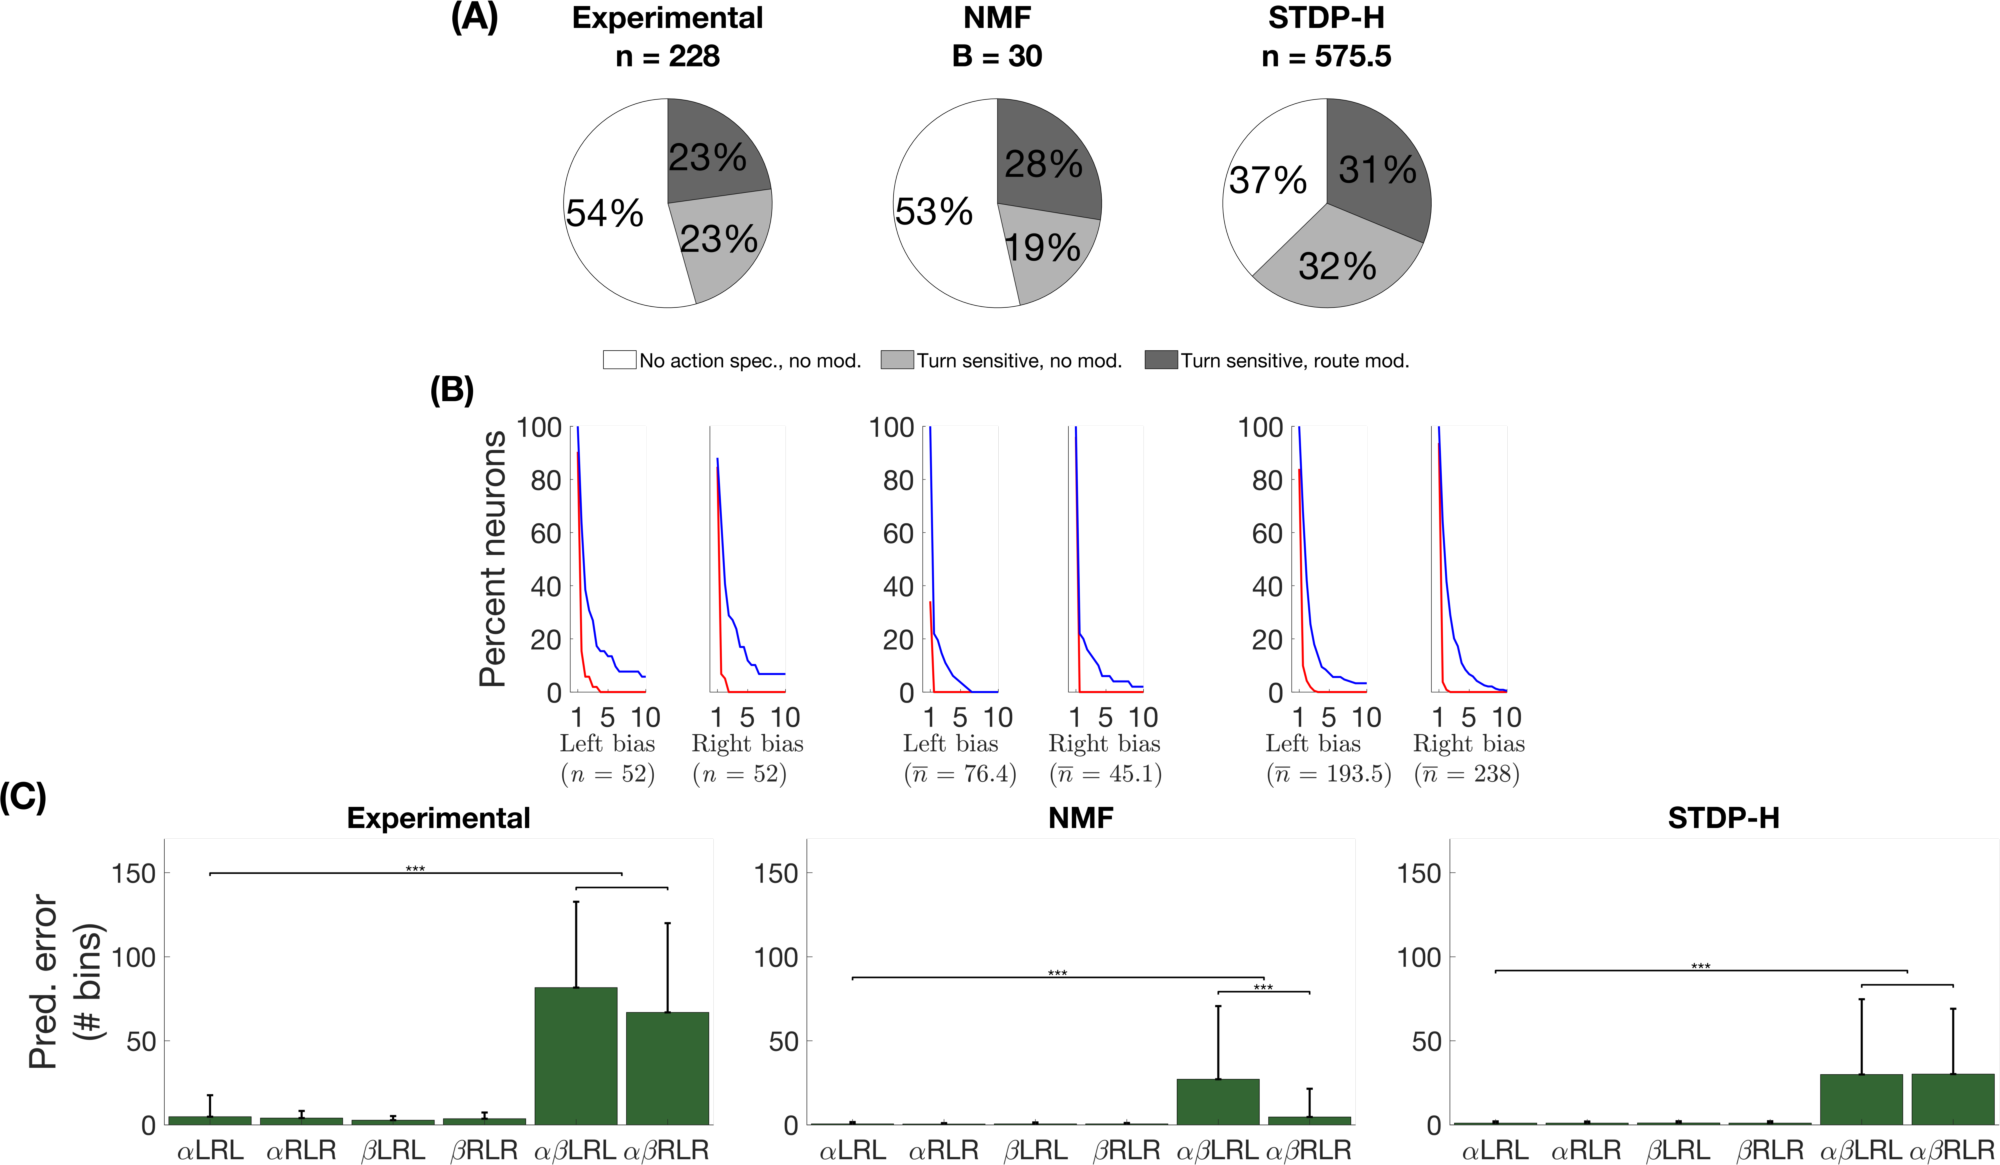
\includegraphics[width=\textwidth]{nmfFig_full}
%     \caption{(A) Neurons in the experimental RSC dataset were classified into three functional categories (turn insensitive, turn sensitive with no route modulation, and turn sensitive with route modulation). Distributions of cell types assigned to each functional category under the NMF and STDP-H paradigms approximate the estimates in the original dataset. (B) Turn sensitive neurons had turn bias ratios, measured as the ratio of activity averaged for all left turn instances vs. for all right turn instances, that were significantly greater than that expected by chance, as determined by cdfs computed using randomized (red line) and non-randomized (blue line) turn identity matrices. Turn bias ratios computed for neurons produced using NMF and STDP-H also had turn bias ratios whose cdfs matched that seen in the experimental data. (C) Ensemble activity across the population could accurately predict the agent's location on the track, demonstrating a sensitivity to the route frame of reference. Reconstructions of position along the route were not as accurate when comparing track positions that occupied different allocentric locations in space ($\alpha$ vs. $\beta$). Sensitivity to both the route-centric and allocentric reference frames were reaffirmed for synthetic neural activity generated under NMF and STDP-H paradigms.}
% 	\label{fig:evidence|RSC}
% \end{figure}
% % END FIGURE

% \cite{Rounds2016} found that the feature conjunction
% exhibited by \ac{RSC} neurons
% could be replicated by evolving a combination of
% \ac{STDP} and homeostasis via synaptic scaling \ac{STDPH}
% that governed the weights of a population of \acp{SNN}.
% The networks were judged by how well the synthetic neural activity patterns matched those seen in the experimental dataset provided by \citep{AlexanderNitz2015}. Four behaviorally relevant variables recorded in tandem with neurophysiological activity were used as inputs to the network by passing each value through an idealized input neuron tuning curve. The variables included angular velocity (AV), linear velocity (AV), head direction (HD), and position (Pos). Gaussian tuning curves were used for AV, LV, and Pos, while a cosine tuning curve was used for HD. The number of idealized input neurons corresponded to the number of tuning curves needed to fully encompass the range of values each behavioral variable could take on. This procedure yielded a total of $417$ input neurons, of which $390$ neurons encoded allocentric position, $7$ neurons encoded angular velocity, $12$ neurons encoded linear velocity, and $8$ neurons encoded head direction. 



% \begin{figure}[t]
% 	\centering
% 	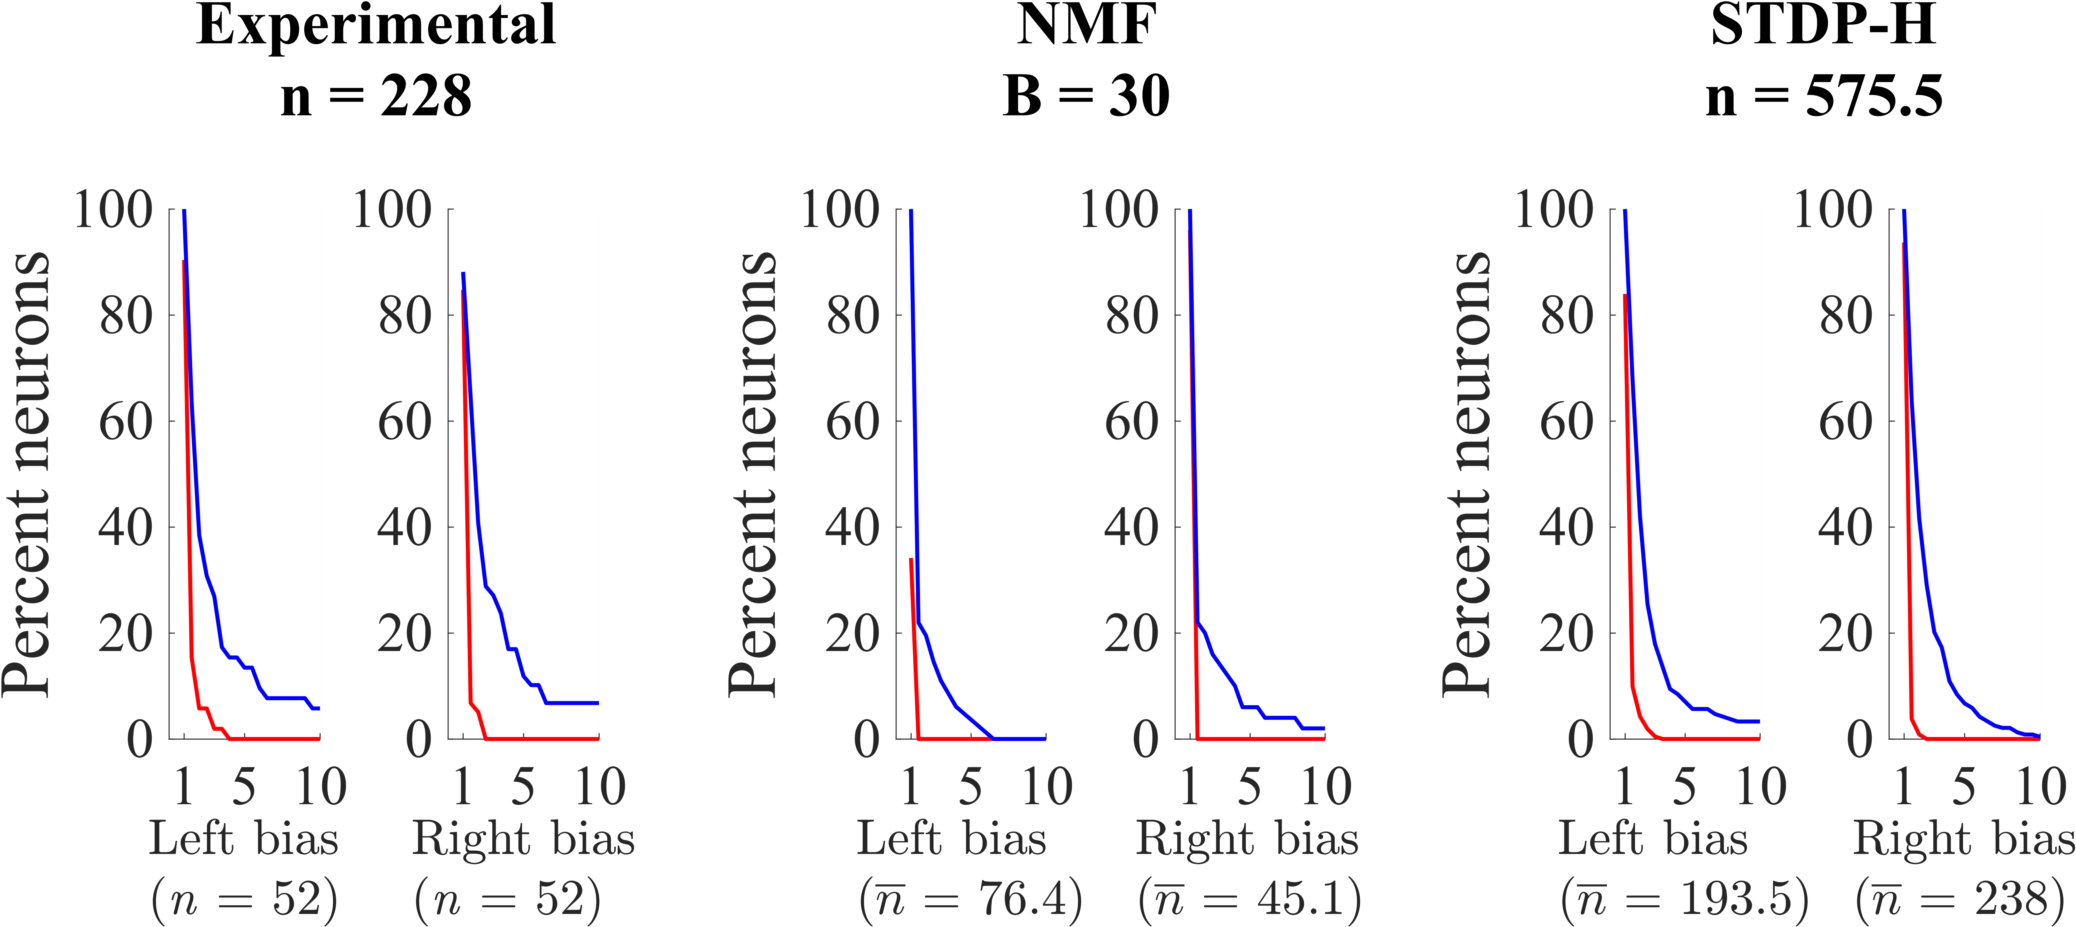
\includegraphics[width=\textwidth]{nmfFig2_turnBiasDists}
%     \caption{In order to examine whether or not turn sensitivity in the population was a product of chance, real and randomized cumulative distribution functions of each neuron's turn bias (ratio of activity for the preferred turn type to the activity of the not preferred turn type) were computed. This involved creating a turn identity matrix that indexed the average activity of the neuron for each instance of both left and right turns, and then averaging the activity for the left turn and right turn sites. Then the ratio was taken between the preferred and non-preferred turn type. Turn biases ranged from 1 to over 10 in some cases. Whether or not these turn biases were a product of chance was tested by randomizing the turn identity matrices over 25 iterations and computing randomized turn bias ratios in the same fashion. Following randomization, cdfs were created for the real and randomized distributions. In the experimental dataset, actual turn bias ratios were significantly above what would be expected by chance, as determined by a Kolmogorov-Smirnov test, p $<$ 0.0001 (left). Similar results were found under both NMF and STDP-H paradigms, suggesting that both methods were able to generate neurons with activity patterns that were tied to the animals' turning behaviors (middle, right).}
% 	\label{fig:evidence|RSC2}
% \end{figure}

% \begin{figure}[t]
% 	\centering
% 	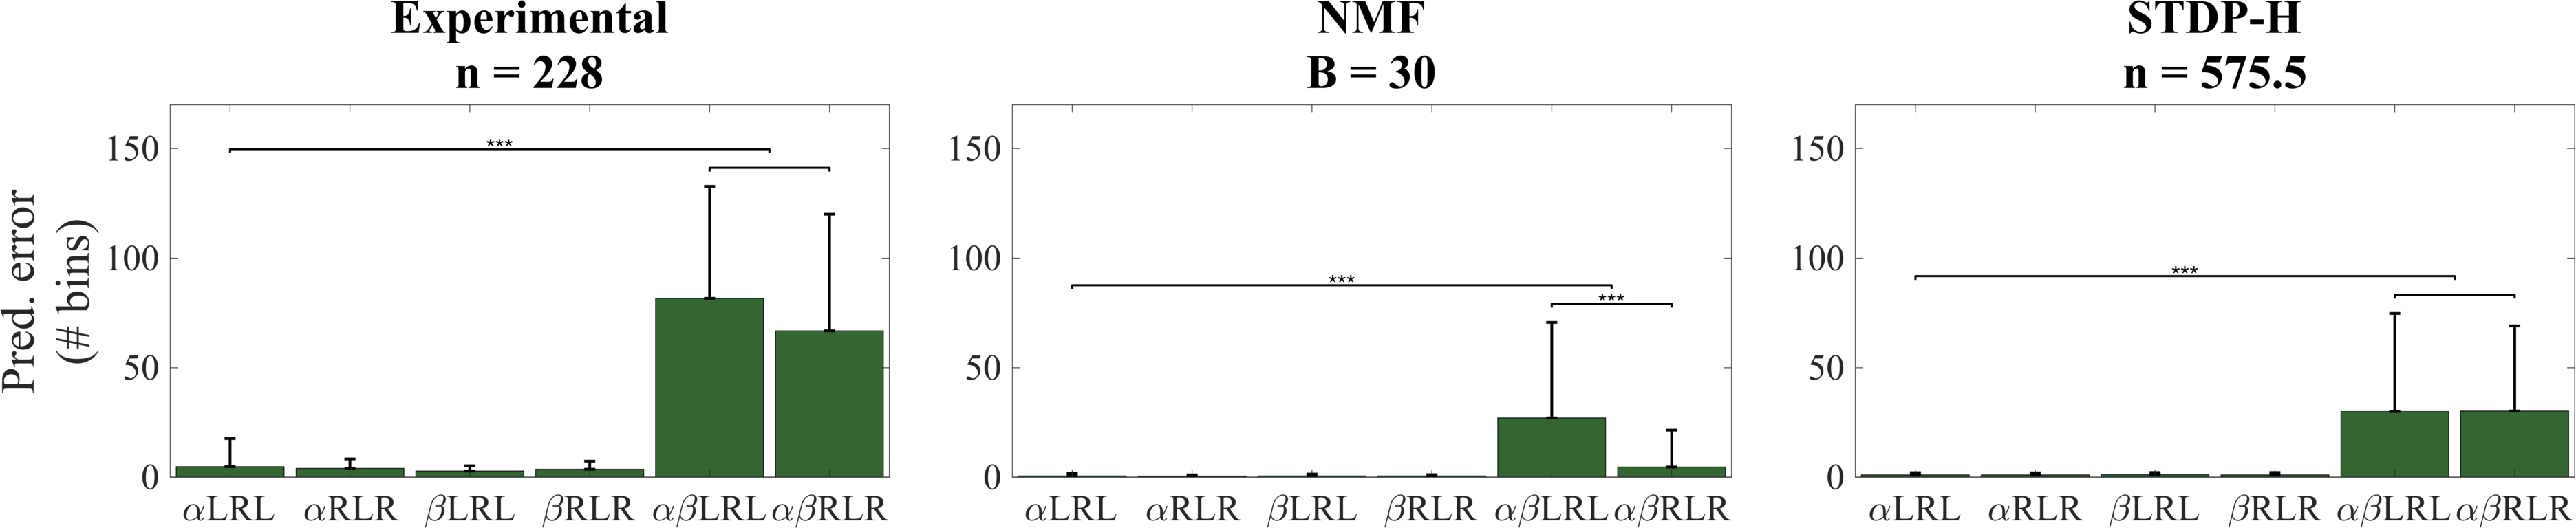
\includegraphics[width=\textwidth]{nmfFig3_reconErrs}
%     \caption{Functionality at the level of the population the RSC dataset was investigated by examining sensitivity to the route-centric and allocentric external frames of reference. Ensemble activity in the RSC is sensitive to both in a conjunctive manner. In the experimental setup, rats completed multiple trials of running back and forth along a W-shaped track that occupied various allocentric positions (x-y coordinates) in the room. Following the experiments, the track was linearized and divided into 200 bins, with each bin being about the length of an adult rat, excluding his tail. To determine sensitivity to the route-based frame of reference, neural activity was averaged across all even trials and all odd trials separately, and then correlation matrices were constructed by correlating the averaged neural activity associated with even trials and the averaged neural activity associated with odd trials. If the neurons encoded the route frame of reference, then the points of highest correlation should occur at the same bins, creating a theoretical perfect prediction line. The actual points of highest correlation were subtracted from this line and the values were averaged to obtain the average reconstruction error. Bar plots of reconstruction error are show in this figure. For even vs. odd trial reconstructions, error was very low (near zero, arbitrary units). However, if the network also encoded the allocentric frame of reference, then correlations between neural activity for tracks that occupied different positions within the room should not yield the same perfect prediction line (that is, correlations should not occur for the same bins, since their positions were different). In the experimental dataset, reconstructions from the two separate track positions, $\alpha$ and $\beta$, yielded much higher error (left), which was found to be significant (Kruskal-Wallis test, p $<$ 0.001). This was again found to be true under the NMF and STDP-H paradigms.  Under NMF, reconstruction error was even lower than in the experimental dataset for even vs. odd trial reconstructions. Error was also comparatively low for reconstructions from $\alpha$ vs. $\beta$, but was found to be significant for both LRL and RLR turn sequences. Error was very low for $\alpha$ vs. $\beta$ reconstructions for the RLR route, but this may have been due to a bias in the dataset that was exploited by NMF (error was slightly lower for $\alpha$ $\beta$ RLR in the experimental dataset as well, but not to such an extreme). Both were nonetheless significantly different, as determined by a Kruskal-Wallis test, p $<$ 0.001, from the even vs. odd trial reconstructions (right). Under STDP-H, results similar to the experimental results were obtained, without a bias that resulted in reduced average reconstruction error for the  $\alpha$ vs. $\beta$ reconstructions.  There was no significant difference between them, but both were significantly different from the even vs. odd trial reconstructions (Kruskal-Wallis test, p $<$ 0.001). Overall, results for STDP-H were similar to the experimental results and similar to results obtained through NMF (right).}
% 	\label{fig:evidence|RSC3}
% \end{figure}

% Because \ac{STDPH} could be used to evolve networks whose behavior matched that observed in the biological retrosplenial cortex, we hypothesized that if ac{STDPH} can approximate \ac{NMF}, then applying \ac{NMF} to the parameterized behavioral variables should yield similar results to the synthetic neural activity observed in the evolved \acp{SNN} under \ac{STDPH}.
% To test this hypothesis, we constructed a virtual input data matrix consisting of the parameterized behavioral variables, whose rows corresponded to the variable type (AV, LV, HD, and Pos), and whose columns corresponded to the observed idealized input firing rates for all trials recorded in the electrophysiological dataset. Half of the trials in the dataset were used as input to the \ac{NMF} algorithm. The basis elements recovered by \ac{NMF} were then interpreted as the synaptic weights of a population of hypothetical \ac{RSC} neurons. By presenting the latter half of the dataset as test input to these hypothetical neurons, the simulated activity of these hypothetical neurons was then analyzed using methods described in \cite{AlexanderNitz2015} to investigate the behavior of the population. What they found was that the model closely matched on several relevant metrics, including functional neuronal type distribution and population behavior (Figure \ref{fig:evidence|RSC}), demonstrating that the population of NMF basis vectors could encode these variables in a manner similar to the biological RSC. Furthermore, 228 recorded RSC neurons were associated with the electrophysiological dataset, but under \ac{NMF} conditions, 30 basis vectors (or $n = 30$) were sufficient to reproduce the behavior of the population.


% \subsection{Dimensionality reduction is not restricted to cortex}
% \label{sec:evidence|bg}

% There is also the strong possibility that some form of dimensionality reduction occurs in subcortical brain regions as well. The striatal-cortical pathway, thought to be involved in reinforcement learning, action selection, and sequence learning, is traditionally viewed in a sequential, feedforward manner: frontal cortical areas transmit information to input regions to the basal ganglia (striatum and subthalamic nuclei (STN)), which project to the globus pallidus, particularly the external part (GPe), which project to output regions of the basal ganglia, including the internal globus palllidus (GPi) and substantia nigra (SNr). The output areas project to the thalamus, which in turn convey information back to frontal cortical regions, completing the loop. More recently, evidence suggests the thalamus also projects back to the striatum and STN. There are two main observations to motivate the idea that some form of dimensionality reduction is required for this region to perform reinforcement learning.
% First, views on the structure and connectivity of the basal ganglia have historically fallen into two camps that argued for the parallelization of the striatal-cortical pathway or for a funnel-like architecture in which information converged at each stage of the pathway, motivated by the observation that the number of neurons decreases dramatically at each stage of the pathway from frontal cortical areas to the GPe. Studies of the region have differed in the absolute numbers present in each area based on species and methodology, but ratios between numbers of neurons have been consistent. From the frontal cortex to the striatum, there is a convergence ratio of ten in which the number of neurons in the frontal cortex number at about $117 x 10^{-6}$, while the neurons in the striatum number at about $1.17 x 10^{-6}$. From the striatum to the internal globus pallidus (GPi) and substantia nigra (SNr), there is a reduction ranging from $10^{2}$ to $10^{3}$ with a factor of converge of about 571 in macaques and 347 in humans. However, it is an open question of how many thalamic neurons receive projections from the GPi and SNr, though indirect evidence suggest increases in the number of connected neurons, suggesting a bottleneck structure.

% Evidence for parallelization comes from anatomical studies and electrophysiological recordings of striatal and pallidal neurons.  Anatomical studies of  trans-neuronal virus transport provide evidence for a parallel macro-organization of the pathway, and  different frontal cortical regions project most densely to distinct regions of the striatum. Early recordings of neurons in the basal ganglia revealed somatotopic organization of structures within the basal ganglia. 

% However, more recent evidence provides support for convergence within the basal ganglia as well. In the afore-mentioned physical studies, the borders between different regions of the basal ganglia were not clearly delineated and many of them overlapped, especially between the striatum and the STN. Furthermore, there is wide dendritic arborization of pallidal neuron, which are oriented at right angles to incoming striatal neurons. There is also a system of collateral synaptic connections in the striatum and pallidum, as well as divergent STN projects to the globus pallidus (GP), with a substantial reduction in the number of neurons between the striatum and GP, which all suggest a convergent structure at the level of the pallidum. In recording studies, careful analysis also revealed at approximately 20\% of recorded striatal neurons responded concurrently to stimulation in the MI and SMA. A considerable number of pallidal neurons were also inhibited by the stimulation of multiple cortical regions, including the frontal cortex, premotor/motor cortex, and supplementary motor and arcuate premotor areas, which should not be the case if each of these frontal regions project to distinct areas in the striatum and striatal-pallidal connections parallelized. Another study used orthodromic stimulation to show that inputs from remote striatal neurons to a focal area in the pallidum followed a funnel-like structure. More recent studies of primates performing complex behavioral tasks revealed a significant proportion of neurons that responded to multiple segregated behavioral events (e.g., limbic, cognitive, and motor). Modern models of the basal ganglia are often a hybridization of parallelized and convergent structure (\ref{sec:evidence|bg}; \cite{BarGad2003_Review}).
% The second observation to motivate the need for dimensionality reduction has to do with the prevalence of anatomical connections that are highly suggestive of lateral inhibition in the basal ganglia. Medium spiny neurons in the striatum terminate within the region onto striatal interneurons and other medium spiny cells. These contacts are GABAergic and ought to indicate lateral inhibition; however, physiological studies have failed to find evidence of such inhibitory interactions and have concluded that functional lateral inhibition in the striatum is weak or nonexistent. Recent studies have employed averaging techniques to enhance the signal to noise ratio and have revealed some inhibitory synaptic potentials, but these are found in less than a third of tested neuron pairs and were unidirectional in most cases, and correlations between their activity have not been found. In the globus pallidus, projecting neurons give rise to specialized dendrites whose purpose are largely unknown . In tissue slices, experimenters have observed IPSPs, which they suggest come from active GP cells within the tissue sample. However, GP to GP synaptic connectivity has only been observed in one out of 40 pairs, and their spiking activity has been uncorrelated.  This raises an important question; since there is extensive anatomical evidence for lateral inhibition in the basal ganglia, particularly the striatum and globus pallidus, but a complete lack of functional lateral connectivity in these same structures, why is the connectivity there? Dimensionality reduction may provide an answer, which is related to the convergent nature of the architecture of the basal ganglia. Relatedly, connectivity in the basal ganglia is very sparse. There are estimated to be around $10^{7}$ cortical-striatal neurons, but a single striatal neuron receives only $10^{4}$ cortical synapses, which means that approximately only 0.01\% of cortical neurons project to the striatum. The same is true for striatal neurons that project to the GP, estimated to be at about 0.1-1\%.

% While computational models of the basal ganglia have either been high-level models of pathology in the region or detailed network models of action selection or sequence learning, all of them have neglected features of the architecture of the basal ganglia, such as the presence of lateral inhibitory connections. Bar-Gad et al. proposed a basic  reinforcement driven dimensionality reduction model of the basal ganglia to explain the presence of lateral inhibitory connections and its convergent structure tho show how the basal ganglia might compress cortical information with respect to a modulatory reinforcement signal. Early iterations of this model featured two layers, used a PCA-based learning rule (Oja's rule) modulated by a scalar reinforcement value and were fully connected, but nonetheless showed that the dynamics of the lateral inhibitory connections lead to complex changes in correlations between neural activity that would explain why no correlations were found following network convergence \cite{BarGad2000}. Initially, output activity would be correlated because multiple output neurons encoded the same aspects of the input; however, over time, the lateral connections caused an orthogonalization of their activity patterns. The model was still able to correctly learn associations between actions and rewards. While the basic model featured only the use of a PCA-based learning rule, an advanced model introduced a sign constraint on the weights in the network, which essentially altered the dimensionality reduction method being used to \ac{NMF}. The network was also made more sparse and incorporated multiple layers, as well as both linear and non-linear neurons \cite{BarGad2003_Review}.

% This model lays the groundwork for two important experiments that might validate the presence of dimensionality reduction techniques in the basal ganglia: While an animal learns to perform a new task, the strength of lateral connections in the striatum and pallidum are expected to increase. By testing either a young animal, or an animal exposed to an entirely new environment, one should see changes in the functional connectivity of the lateral inhibitory connections since different motor and sensory mappings are expected to alter the structure of the input space. Secondly, Hebbian, anti-Hebbian, and reinforcement learning rules are predicted to be found in the basal ganglia, but have yet to be documented.  If these two predictions are confirmed, then it is possible that some form of dimensionality reduction, possibly \ac{NMF}, occurs in this brain region.

% Perhaps put this last, because it is subcortical.
% Tone: NMF might even happen in subcortical structures. For example, in the basal ganglia,
% there is evidence for blah blah...
% But check the literature: Is RDDR more like PCA (holistic representation)? Or is it by
% any chance sparse or parts-based?

% There’s an interesting idea that the basal ganglia might be doing reinforcement-driven dimensionality reduction (RDDR), by compressing cortical information according to a reinforcement signal using optimal extraction methods (Bar-Gad et al. 2000).
% It might be worth doing a forward search on RDDR.
% There’s a good high-level summary of the Bar-Gad study in the review of (Joel, Niv, and Ruppin 2002).

